%% content.tex
%%

%% ==============================
\chapter{Prelude}
\label{ch:Introduction}
%% ==============================

\section{Abstract}

\vspace*{\fill}
Die Strahlverfolgung und dazugehörige Techniken gewinnen gegenwärtig in der Echtzeitcomputergrafik an Bedeutung. Dabei haben bereits frühere Arbeiten
die blue noise Fehlerverteilungen miteinbezogen und deren Bedeutung in der Steigerung der wahrnehmbaren Bildqualität hervorgehoben und verdeutlicht.
Diese Arbeit wird diesen Stand aufnehmen und einen zeitlich stabilen Algorithmus erläutern. Ein Algorithmus, der mit Anzahl der Samples und Dimension
des Tracers einhergeht. Im Gegensatz zu vorhergehenden Ansätzen wollen wir direkt im Bildraum eine Fehlerumverteilung anwenden, um so eine entsprechend 
korrelierte Pixelfolge zu erhalten. All dies erreicht der Algorithmus ohne signifikanten Mehraufwand.
\vfill

\newpage

\section{Einleitung}
\vspace*{\fill}
Dithering ist in Echtzeitanwendungen bereits verbreitet. So zu sehen in dem Computerspiel \textit{Call of Duty: Advanced Warfare}, wobei 
bereits im Post-Processing \cite{callofdutypostprocessing} mit white noise und bayer pattern gearbeitet wird.\par 
Weitere Entwicklungen \cite{georgiev2016blue} haben sich mit blue noise dither masks \nameref{ch:Content1:sec:BlueNoise} beschäftigt
und ihre Nützlichkeit in Steigung der visuellen Qualität gezeigt. Hierbei lassen sich im Bildraum die entstehenden 
Monte-Carlo-Integrationsfehler \nameref{ch:Content1:sec:PathTracer} zwar nicht verringern, jedoch umverteilen.\par 
Im Besonderen zeigte \cite{Sch19} die Bedeutung von blue noise Fehlerverteilung im Bildraum für Echtzeitanwendungen mit neuer
Raytracingtechnologie.
Das vor dem temporalen Algorithmus erschienene Paper \cite{heitz:hal02150657} zeigt eindrucksvoll die Mächtigkeit von 
Fehlerumverteilungen im Bildraum. 
Die Entwickler von INSIDE \cite{10.111712.152707} fanden auch bereits eine Anwendung für blue noise Fehlerverteilungen. 


\vfill
%% ==============
\chapter{Grundlagen}
\label{ch:Grundlagen}
%% ==============


%% ===========================
\section{Path Tracer}
\label{ch:Content1:sec:PathTracer}
\subsubsection{Funktionsweise}
Bei der Bilderzeugung, ausgehend von Szenen, welche viel Geometrie beinhalten bzw. bei Szenen 
die generelle BRDF's verwenden eignet sich das \ref{ch:Content1:sec:PathTracer}path tracing \cite{kajiya1986rendering}.
Das \ref{ch:Content1:sec:PathTracer}path tracing ist in Hinsicht der Beleuchtung komplett. Deshalb lässt sich damit
\textit{Global Illumination} erreichen. Das hier verwendete \ref{ch:Content1:sec:PathTracer}path tracing in 
\cite[eragae]{Benty18} verwendet eine klassische Umsetzung.\par

\begin{figure}[H]
    \centering
    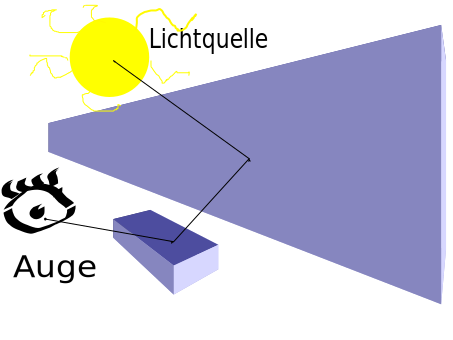
\includegraphics[width=0.7\linewidth]{content/PathTracer/Bilder/Grundkonzept_path_tracing.pdf}
    \label{pic::PathTracingGrundkonzept}
    \caption{Grundkonzept path tracer}
\end{figure}


Wie in \cite{marschner2009fundamentals} beschrieben wird ausgehend von der vollständigen Transportgleichung
\begin{equation}\label{eq:vollstaendige Transportgleichung}
    L_s(k_0) = L_e(k_0) + \int_{all(k_i)}^{} \rho(k_i, k_0)*L_f(k_i)*cos(\theta_i)d\theta_i
\end{equation}
    
\begin{equation}\label{eq:kajiya}
        I(x,{x}^{'}) = g(x,{x}^{'}) * \biggl[\epsilon(x,{x}^{'}) + 
                        \int_{S}^{} \rho(x,{x}^{'},{x}^{''})
                        I({x}^{'},{x}^{''}d{x}^{''})\biggr] 
\end{equation}
Sie beschreibt den Energietransport \textit{I} von einem Punkt ${x}^{'}$
zu einem Punkt x. Dabei ist ein maßgebender Faktor der Geometrieterm \textit{g},
der die relative Lage der beiden Punkte zueinander im Raum beschreibt.
Ein weiterer Faktor ist die Abstrahlung \textit{$\epsilon$} von ${x}^{'}$ nach x. 
Beeinflusst wird der Energiefluss auch durch
die bidirektionale Verteilungsfunktion \textit{$\rho$}, welche Aufschluss über
das einfallende Licht von einem Punkt ${x}^{''}$ über ${x}^{'}$ zu x gibt.\par
Die Schlussfolgerung aus dieser Gleichung \ref{eq:kajiya} ist: Die transportierte
Intensität von einem Licht zu einem Anderen ist die Summe des ausgestrahlten Lichts 
und das ausgestrahlte Licht zu x von allen anderen Oberflächen.


\subsubsection{Monte-Carlo-Integration}
Mit der Monte Carlo Integration approximieren wir die Rendergleichung.\par 
Bei gegebener Funktion \textit{f }:\textit{ S}$\rightarrow \mathbb{R}$ und der 
Wahrscheinlichkeitsdichtefunktion $x \sim p$
\cite{KK02}
\label{pic:MonteCarloIntegration}
\begin{equation}\label{eq:montcarlo}
    \int_{x\in S} g(x) d\mu \simeq \frac{1}{N}*\sum_{i=1}^{N}\frac{g(x_i)}{p(x_i)}
\end{equation}

\begin{figure}[H]\label{pic:WeissesRauschenTracer}
    \centering
    \begin{minipage}[t]{0.45\linewidth}
        \centering
        \includegraphics[width=\linewidth]{content/PathTracer/Bilder/WeissesRauschenSzene.png}
        \caption{Szene mit Weißem Rauschen}
    \end{minipage}
    \hfill
    \begin{minipage}[t]{0.45\linewidth}
        \centering
        \includegraphics[width=\linewidth]{content/PathTracer/Bilder/FFT_Ausschnitt2.png}
        \caption{FFT des Ausschnitts}
    \end{minipage}
\end{figure}




%% ===========================


%% ===========================
\newpage
\section{Blue Noise}
\label{ch:Content1:sec:BlueNoise}
\subsection{Eigenschaften}

Wie in \cite{Pet17} vorgestellt, macht man sich die Eigenschaften einer
blue noise Textur zu Nutze. Dabei werden im Folgenden, die dort bereit 
gestellten blue noise verteilten Texturen verwendet, welche anhand des in
\cite{ulichney1993void} vorgestellten Algorithmus erstellt wurden.
Die korrespondierenden Spektren werden mit Hilfe von \cite{FFTProgWeb} erstellt.

\subsubsection{Uniformität}
Die Uniformität(lat. \textit{uniformitas}-Einförmigkeit) garantiert uns 
wie in \cite{3288} eine gleichverteilte Wahrscheinlichkeitsdichtefunktion
mit zugehöriger gleichverteilter Wahrscheinlichkeitsfunktion. In \cite{Pet17}
sieht sie wie folgt aus: 

\begin{equation}\label{eq:uniformität}
    P(n \leq p) = p
\end{equation}

\subsubsection{Niedrige Frequenzen}
Niedrige Frequenzen sind in einer blue noise sehr wenig bis gar nicht 
vertreten. Dies ist an dem schwarzen Ring innerhalb der Fouriertransformierten
zu erkennen\ref{pic:blueNoiseFFT}.

\begin{figure}[H]\label{pic:blueNoiseFFT}
    \centering
    \begin{minipage}[t]{0.45\linewidth}
        \centering
        \includegraphics[width=\linewidth]{content/BlueNoise/Bilder/LDR_LLL1_0.png}
        \caption{$512^{2}$ blue noise Textur}
    \end{minipage}
    \hfill
    \begin{minipage}[t]{0.45\linewidth}
        \centering
        \includegraphics[width=\linewidth]{content/BlueNoise/Bilder/FFT_LDR_LLL1_0.png}
        \caption{Fourier Spektrum $512^{2}$ blue noise Textur}
    \end{minipage}
\end{figure}

\begin{figure}[H]\label{pic:bayerPatternFFT}
    \centering
    \begin{minipage}[t]{0.45\linewidth}
        \centering
        \includegraphics[width=\linewidth]{content/BlueNoise/Bilder/BayerMatrix.png}
        \caption{$512^{2}$ bayer pattern Textur}
    \end{minipage}
    \hfill
    \begin{minipage}[t]{0.45\linewidth}
        \centering
        \includegraphics[width=\linewidth]{content/BlueNoise/Bilder/FFT_BayerMatrix.png}
        \caption{Fourier Spektrum $512^{2}$ bayer pattern Textur}
    \end{minipage}
\end{figure}

\begin{figure}[H]\label{pic:tiledBlueNoiseFFT}
    \centering
    \begin{minipage}[t]{0.45\linewidth}
        \centering
        \includegraphics[width=\linewidth]{content/BlueNoise/Bilder/BlueNoise64Tiled.png}
        \caption{$512^{2}$ bayer pattern Textur}
    \end{minipage}
    \hfill
    \begin{minipage}[t]{0.45\linewidth}
        \centering
        \includegraphics[width=\linewidth]{content/BlueNoise/Bilder/FFT_BlueNoise64Tiled.png}
        \caption{Fourier Spektrum $512^{2}$ bayer pattern Textur}
    \end{minipage}
\end{figure}

\subsubsection{Isotropie}
Die Isotropie(altgr. \textit{isos}-gleich und \textit{tropos}-Richtung)
einer blue noise Textur wird ausgenutzt. Dabei haben wir in allen
Dimensionen (in dieser Arbeit werden Texturen mit zwei benutzt) 
die Unabhängigkeit einer Eigenschaft. 


\subsubsection{Kachelung}
Eine weitere nützliche Eigenschaft der blue noise Verteilung ist die 
Möglichkeit der Kachelung. 
%% ===========================

%% ===========================
\newpage
\section{Blue Noise Sampling}
\label{ch:Content1:sec:BlueNoiseSampling}
%Betrachten wir Verfahren wie das \nameref{sec:quasi monte carlo} Verfahren, 
\label{subsec:dither sampling}
Nachdem wir die Eigenschaften der \nameref{ch:Content1:sec:blue noise} kennengelernt haben
können wir zusammen mit dem Verständnis über den \nameref{ch:Content1:sec:Path Tracer} und der 
zugrundeliegenden Monte-Carlo Integration \ref{eq:Monte-Carlo} das dithered sampling verstehen.
\textit{Dithering} ist das bewusste Einbringen eines Rauschens um entstehende Quantisierungsfehler
zu randomisieren \cite{georgiev2016blue}.
Klassischerweise wird eine zweidimensionale 
\nameref{ch:Content1:sec:blue noise} Textur verwendet um mit einer darauf aufbauenden Schwellenwertbildung
dieses Rauschen in ein Bild zu bringen. 
Hier wollen wir durch Dithering die Verteilung des 
entstehenden Monte-Carlo Integrationsfehlers verändern.\par
Grundlage des d-dimensionalen \nameref{ch:Content1:sec:Path Tracer} werden sowohl eine 
\nameref{ch:Content1:sec:blue noise}-Verteilung als auch Anfangswerte $s_{n}$ gleicher Dimension.
Damit konkretisiert sich die Monte-Carlo Integration \ref{eq:Monte-Carlo} mit Integrand f zu folgender 
Gleichung:
\begin{equation}\label{eq:concreteMonteCarlo}
    \frac{1}{N}\sum_{n=0}^{N-1}f(s_{n})
\end{equation}

\cite{georgiev2016blue} hat sich mit einer direkten Korrelation der Anfangswerte anhand einer 
\nameref{ch:Content1:sec:blue noise} Textur beschäftigt, in der Hoffnung das der Integrand f diese
Verteilung behält. \cite{hal02158423} zeigt jedoch die Limitierung dieser Methode auf und 
formuliert eine \nameref{ch:Content2:sec:a Posteriori}-Methode, welche wir uns für den 
Temporalen Algorithmus \ref{ch:Temporaler Algorithmus} zu Nutze machen werden.




%% ===========================

%% ===========================
\newpage
\section{Quasi-Zufallsfolgen}
\label{ch:Content1:sec:QuasiRandomSequences}
Sobol \cite{owen1998scrambling} \cite{heitz:hal-02150657} \cite{quasirandomsequencesbyRoberts}
\todo{find appropriate information and add it}

%% ===========================


%% ===========================
\section{Simulated Annealing}
\label{ch:Content2:sec:SimulatedAnnealing}
Im vorherigen Kapitel, dem Retargeting Schritt \nameref{ch:Content2:sec:Retargeting},
wird eine vorberechnete Retargeting-Textur verwendet. Diese speichert eine
Permutation, die unsere blue noise Textur vom frame t in eine
blue noise Textur vom frame t+1 umwandelt. Diese Permutation wird 
dann auf die Startwerte angewandt bevor das nächste frame t+1 gerendert wird.
Dadurch werden die blue noise Umverteilung der Sorting Phase \nameref{ch:Content2:sec:Sorting}
akkumuliert und die optische Aufwertung erst richtig sichtbar.
Die retarget Textur wird mit Hilfe von \textbf{simulated annealing} 
\cite{hal02158423} berechnet. Wir wollen somit eine approximativ 
optimale Lösung finden: Permutiere Pixel der blue noise Textur von 
frame t bis Sie sehr ähnlich verteilt sind wie die Pixel der blue noise
Textur von frame t+1. Dabei ist die Lokalität der Vertauschungen, 
welche wir bereits in der Sorting Phase\nameref{ch:Content2:sec:Sorting}
verwendet haben, wichtig.

Die Funktion nach der optimiert wird ist an die Formel aus\cite{georgiev2016blue} angelehnt.
\begin{equation}\label{eq:pixel energy function}
    E(M) = \sum_{p \neq q}E(p,q) = 
           \sum_{p \neq q} \mathrm{e}^{-\frac{\Vert{p_{i}-q_{i}}\Vert^{2}}{\sigma_{i}^{2}} -
           \frac{\Vert{p_{s}-q_{s}}\Vert^{d/2}}{\sigma_{s}^{2}}}
\end{equation}
Wähle nach \cite{ulichney1993void} $\sigma_{i} = 2.1$ und $\sigma_{s} = 1$ 
Zu den Pixeln p,q beschreibt $p_{i}$ und $q_{i}$ ihre jeweiligen Koordinaten.
Und $p_{s}$ und $q_{s}$ sind ihre d-dimensionalen Samplewerte.


\begin{algorithm}[H]
    \caption{\textbf{Simulated Annealing} finde sehr gute Lösung}
    \begin{algorithmic}[1]
        \State initialisiere Startzustand $s=s_{0}$
        \For{i=1...maxSteps}
        \State //Radius für Nachbarschaftssuche ist auf 6 festgesetzt
        \State $s_{neu}\leftarrow$Nachbarzustand(s)
        \If{P(Energie(s), Energie($s_{new}$))$\ge$ random(0,1)} 
        \State s = $s_{new}$
        \EndIf
        \EndFor
        \State return Endzustand s;
    \end{algorithmic}
    \label{alg:retargeting}
\end{algorithm}

Als Startzustand $s_{0}$ definieren wir eine Permutation, die alle 
Elemente auf sich selbst abbildet.
Um von einem Zustand s zu einem neuem Zustand $s_{new}$ zu kommen,
definieren wir eine Nachbarschaftsfunktion \textit{Nachbarzustand()}. 
Diese kann zwei Elemente genau dann vertauschen, wenn Sie in einem 
gegenseitigen Radius r = 6 erreichbar sind. Dabei vertauschen wir
in jedem Schritt ein Pixelpaar. 
Die Wahrscheinlichkeitsfunktion zur neuen Zustandsannahme
P(Energie(s), Energie($s_{new}$)) beschreibt, ob wir den neu
gewählten Zustand $s_{new}$ übernehmen. Dabei wird klassischerweise die
Akzeptanz von Zuständen mit höherer Energie immer kleiner.(bzw. die 
Toleranz gegenüber größeren Fehlern im Bezug zur Zeit). Die allgemeine Akzeptanz von 
Zuständen mit höherer Energie ist dabei von fundamentaler Bedeutung.
Somit verlassen wir möglicherweiße nur lokale Maxima.
Die zu minimierende Energiefunktion E\nameref{eq:pixel energy function} betrachtet
dabei zwei 

\begin{figure}[H]\label{pic:Retargeting}
    \centering
    \begin{minipage}[t]{0.45\linewidth}
        \centering
        \includegraphics[width=\linewidth]{content/simulatedAnnealing/Bilder/LDR_RGBA_64.png}
        \caption{Blue noise Textur 64x64}
    \end{minipage}
    \hfill
    \begin{minipage}[t]{0.45\linewidth}
        \centering
        \includegraphics[width=\linewidth]{content/simulatedAnnealing/Bilder/LDR_RGBA_64_retarget_texture.png}
        \caption{Permutation; gespeichert in R,G-Channel einer .png}
    \end{minipage}
\end{figure}


%% ===========================


%% content.tex
%%

%% ==============
\newpage
\chapter{Temporaler Algorithmus}
\label{ch:TemporalerAlgorithmus}
In diesem Abschnitt wird auf den in \cite{hal02158423} vorgestellten, temporalen Algorithmus eingegangen.
Dieser besteht grundsätzlich aus dem \nameref{ch:Content2:sec:Sorting} sowie den 
\nameref{ch:Content2:sec:Retargeting}. Es sollte unbedingt beachtet werden, dass folgende
Annahmen getroffen wurden: Der Algorithmus arbeitet Blockweise auf den Pixeln und erwartet, dass benachbarte
Pixel innerhalb dieses Blockes den selben Wert haben. Da wir einen temporalen Algorithmus haben, soll diese Annahme 
auch über mehrere gerenderte Bilder hinweg gelten. Es sollte also beachtet werden, dass der Algorithmus z.B. nicht 
für Objektkanten oder ruckartige Bewegungen (der Kamera oder Objekte) ausgelegt ist.
\cite{heitz:hal-02150657}

\cite{quasirandomsequencesbyRoberts}
\todo{find the right place for this chapter}\label{code:golden_ratio}
\begin{lstlisting}[style=CStyle]
   float g = 1.32471795724474602596; //Plastische Zahl
   float a1 = 1.0/g;
   float a2 = 1.0/(g*g);
   x[n] = (0.5+a1*n) %1; //toroidally shifted
   y[n] = (0.5+a2*n) %1; //toroidally shifted
\end{lstlisting}
Die sogenannte Plastische Zahl in \ref{code:golden_ratio} ist die Lösung der
Gleichung \ref{eq:plasticnumber}
\begin{equation}\label{eq:cubic}
   x^{3} - x - 1 = 0
\end{equation}
Die Lösung dieser Gleichung lässt sich über die Padovan und Perrin Sequenz
definieren. Damit erhalten wir Plastische Zahl $\Phi$:

\begin{equation} \label{eq:plasticnumber}
   \Phi = \frac{(9 - \sqrt{69})^{1/3} + (9 + \sqrt{69})^{1/3}}
               {2^{1/3}3^{2/3}}
\end{equation}

\todo{add further information and references!!!}
\cite{vanderlaanplasticnumber}
\cite{wolframalphaPlastic}

%% ==============



%% ===========================
\section{A Posteriori}
\label{ch:Content2:sec:APosteriori}
Um das in Abschnitt \ref{subsec:dither sampling} vorgestellte \textit{Dither Sampling} zu realisieren
benutzen wir für den temporalen Algorithmus \ref{ch:Temporaler Algorithmus} diese im Folgenden vorgestellten
\glqq nachträglichen\grqq Annahmen \cite{hal02158423}. 
A Posteriori sind Sie in dem Sinne, als das wir die Annahmen szenenabhängig machen und Sie anhand 
von bereits erstellten Pixelwerten formulieren. 

\subsection{Theoretische Grundlage}

Im Kapitel \nameref{ch:Content1:sec:Path Tracer} haben wir gesehen, dass 
wir den Wert eines Pixels (i,j) klassischerweise mit einem zufälligen
Startwert durch eine Monte-Carlo Integration erhalten. Wir betrachten im
Folgenden eine (theoretische) Menge von allen möglichen Werten eines 
Pixels, welche durch alle möglichen Startwerte generiert wurde.
In Abbildung \ref{eq:Pixel Schätzung Wahrscheinlichkeitsdichtefunktion} ist die Wahrscheinlichkeitsdichtefunktion
$h_{ij}$ aufgetragen, als eine Funktion über alle möglichen Werte 
$I_{ij}$ eines Pixels (i,j).

\begin{equation}\label{eq:Pixel Schätzung Wahrscheinlichkeitsdichtefunktion}
    H_{ij}([I_{Anfang},I_{Ende}]) = \int_{I_{Anfang}}^{I_{Ende}} h_{ij} dI
\end{equation}

Verfolgt man beispielhaft die Werte eines Pixels über neun Bilder bei unseren \nameref{ch:Content1:sec:Path Tracer}, 
so ergibt es sich zur Anschauung wie folgt:

\begin{figure}[H]

    \begin{subfigure}{\textwidth}
        \centering \includegraphics[width=0.6\linewidth]{content/TemporalerAlg/Bilder/APosteriori/frame_t_whitenosie2.0.png} 
        \caption{Szenenausschnitt}
        \label{fig:szene_pixel_position_512x512}
    \end{subfigure}

    \begin{subfigure}{0.5\textwidth}
        \centering \includegraphics[width=0.6\linewidth]{content/TemporalerAlg/Bilder/APosteriori/pixel_512x512_strip.png} 
        \caption{Werte des Pixels an Position 512x512 im zeitlichen Verlauf (grüner Pfeil)}
        \label{fig:ausschnitt_pixelstrip}
    \end{subfigure}
    \begin{subfigure}{0.5\textwidth}
            \centering
            \def\svgwidth{\columnwidth}
            \import{content/TemporalerAlg/Bilder/APosteriori/}{histogram_of_estimates.pdf_tex}
            \caption{Histogram der Pixelschätzungen}
            \label{pic:histogramOfEstimates}
    \end{subfigure}
        \caption{Pixelwerte an Position 512x512(grüne Markierung) in aufeinanderfolgenden Zeitschritten}
        \label{fig:Pixelwerte}

\end{figure}

Betrachten wir die theoretische, praktisch nicht umsetzbare Menge aller möglichen Werte. 
Mit dieser Menge haben wir ein vollständiges Histogramm. Dies bedeutet wiederrum, dass das Erzeugen eines 
Pixelwertes nichts anderes bedeutet, als eine zufällige Wahl anhand der impliziten
Wahrscheinlichkeitsdichtefunktion. Wir können als einem zufälligen Anfangswert einen konkreten 
Pixelwert zuteilen und eine umkehrbare Funktion definieren \ref{eq:inverse Funktion}. 

Daraus lässt sich die Gleichbedeutung zweier Aussagen begründen:
Das Rendern des Pixels (i,j) und das Wählen eines Pixelswertes $I_{ij}$
von unser zuvor formulierten Wahrscheinlichkeitsdichtefunktion $h_{ij}$.

\begin{equation}\label{eq:inverse Funktion}
    I_{ij} = H_{ij}^{-1}(x), x \in [0,1]
\end{equation}

\par

\textbf{Fazit}: Falls $x \in d_{ij}$, wobei d eine korrelierte Zahlenfolge, die einer 
\nameref{ch:Content1:sec:blue noise} Verteilung entspricht, folgt aus der bijektiven
Natur der Gleichung \ref{eq:inverse Funktion} eine \nameref{ch:Content1:sec:blue noise} 
Fehlerverteilungen im Bildraum. 

Anmerkung: Das Dies nur theoretisch möglich und gerade für Echtzeitanwendungen nicht umsetzbar ist, 
folgt eine praktikable Formulierung!

\subsection{Praktische Durchführung}

Die Berechnung des vollständigen Histogramms ist für eine Echtzeitanwendung
zu kostenintensiv. Stattdessen könnte man auch die dadurch beanspruchte 
Rechenleistung auf z.B mehrere Samples pro Pixel verteilen und dadurch eine 
Steigerung der Bildqualität erreichen!
Stattdessen werden wir in dem temporalen Algorithmus (siehe \cite{hal02158423})
das Histogramm mit dem vorherigen Bild approximieren. 
Die Approximation des Histogramms erfolgt dadurch mit dem $Frame_{t}$ 
für $Frame_{t+1}$. Daher ist eine getroffene Annahme, um die gute Funktionalität des 
Algorithmus zu garantieren, eine nicht zu schnelle Bewegung der Kamera.
Außerdem werden für das Histogramm eines Pixels seine umliegenden benachbarten Pixel gewählt.
Daher ist eine weitere getroffene Annahme, um die gute Funktionalität des 
Algorithmus zu garantieren, eine möglichst homogene Fläche. 
Offensichtliche Konsequenzen dieser blockweisen Verarbeitung sind schlechte blue noise 
Fehlerverteilungen im Bildraum bei sich stark ändernden Bildausschnitten
(so z.B. bei Objektkanten), da dort die Annahme, dass eine ähnliche Oberfläche
zur Farbgebung beiträgt verletzt wird.

\begin{figure}[H]
    \centering
    \begin{subfigure}[b]{0.4\textwidth}
        \centering \includegraphics[interpolate=false, width=\linewidth]{content/TemporalerAlg/Bilder/APosteriori/homogener_ausschnitt_blocksize.png}
        \caption{homogener Pixelblock}
        \label{fig:homogener Pixelblock}
    \end{subfigure}
    \begin{subfigure}[b]{0.4\textwidth}
        \centering \includegraphics[interpolate=false,width=\linewidth]{content/TemporalerAlg/Bilder/APosteriori/inhomogener_ausschnitt_blocksize.png}
        \caption{inhomogener Pixelblock}
        \label{fig:Inhomogener Pixelblock}
    \end{subfigure}

    \caption{Pixelblöcke bei (in-)homogenen Flächen}\label{fig:Pixelblöcke}
\end{figure}

In Abbildung \ref{fig:Inhomogener Pixelblock} sind die benachbarten Pixel eine gute 
Approximation des jeweiligen Pixels, wohingegen in Abbildung \ref{fig:homogener Pixelblock}
die benachbarten Pixel dies nicht sind.
%% ===========================



%% ===========================
\section{Sorting}
\label{ch:Content2:sec:Sorting}
In diesem Schritt wollen wir nun die Untersuchungen aus 
\ref{ch:Content2:sec:APosteriori} durchführen. Nach dem Rendern eines
Frames t(vor dem Rendern von Frame t+1) approximieren wir das Histogramm
der Pixelwerte anhand der Pixelwerte von Frame t.
\cite{hal02158423}
\begin{algorithm}[H]
    \caption{\textbf{Sortier Schritt t} nach dem Rendern von Frame t
    und vor dem Rendern von Frame t+1}
    \begin{algorithmic}[1]
        \STATE pixel \textbf{consists of} value,index;
        \STATE List framePixelsIntensities, noiseIntensities;
        \STATE $assert(sizeof(framePixelsIntensities)==BLOCKSIZE)$;
        \STATE $assert(sizeof(noiseIntensities)==BLOCKSIZE)$;
        \STATE List L $\leftarrow$ pixels of frame t in block;
        \STATE \hfill
        \STATE //init lists
        \STATE initList(framePixelsIntensities, pixelIntensity(L);
        \STATE $blueNoise_{t}$ = calcCorrectOffset(incomingbluenoisetexture);
        \STATE initList(noiseIntensities, pixelIntensity($blueNoise_{t}$));
        \STATE \hfill
        \STATE //sort the two lists by means of intensities
        \STATE sort(framePixelsIntensities);
        \STATE Sort(noiseIntensities);
        \STATE \hfill
        \STATE //now we reorder our seeds hence the sorted lists
        \FORALL{$i = 1 .. BLOCKSIZE$}
        \STATE $sortedSeeds(noiseIntensities.getIndex(i)) = incomingSeeds(framePixelIntensities.getIndex(i))$;
        \ENDFOR
    \end{algorithmic}
    \label{alg:Sortier}
\end{algorithm}
%% ===========================



%% ===========================
\section{Retargeting}
\label{ch:Content2:sec:Retargeting}
\cite{hal02158423}

Zu Grunde liegender Sinn dieses Schrittes: Vertauschen der Anfangswerte, die 
verteilt sind wie $BlueNoise_{t}$, sodass Sie verteilt sind wie die 
$BlueNoise_{t+1}$. Aufgrund dessen haben wir eine Aufsummierung der
blue noise Fehlerverteilungen über viele Frames.

\begin{algorithm}[H]
    \caption{\textbf{Retargeting Schritt} t Vor Rendern Frame t+1 nach Sortier Schritt}
    \begin{algorithmic}[1]
        \State //permutation indices from precomputed texture
        \State $retaget_{t}$ = retargettexure[calcCorrectOffset(incomingbluenoisetexture)];
        \State List<PixelPermutation> L = $retaget_{t}$
        \For{i = 1 .. numberOfPixelsPerBlock}
        \State $retargetedSeeds(L.getNewIndices()) = incomingSeeds(L.getOldIndices());$
        \EndFor
    \end{algorithmic}
    \label{alg:retargeting}
\end{algorithm}

%% ===========================



